\usepackage{ifthen}

% Define an agenda item
%
% Arguments:
% 1: Identifier of the agenda item, should be all lower-case
% 2: Type of the agenda item: lecture or lab
% 3: English title of the agenda item
% 4: English full description of the agenda item
% 5: French title of the agenda item
% 6: French full description of the agenda item
\newcommand\defagendaitem[6]{
  \ifthenelse{\equal{\agendalanguage}{french}}{
    \expandafter\def\csname #1@#2@title\endcsname {#5}
    \expandafter\def\csname #1@#2@contents\endcsname {#6}
  }{
    \expandafter\def\csname #1@#2@title\endcsname {#3}
    \expandafter\def\csname #1@#2@contents\endcsname {#4}
  }
}

% Show/render an agenda item
%
% Arguments:
% 1: Identifier of the agenda item, as defined by \defagendaitem
% 2: Type of the agenda item: lecture or lab
\newcommand\showagendaitem[2]{%
  \ifthenelse{\boolean{hlineneeded}}{\\\hline}{\setboolean{hlineneeded}{true}}%
    \ifthenelse{\equal{\agendalanguage}{french}}{%
      \ifthenelse{\equal{#2}{lecture}}%
      {Cours &}%
      {%
        \ifthenelse{\equal{#2}{lab}}{%
          \ifthenelse{\equal{\trainingtype}{online}}{Démo &}{TP &}%
        }%
        {}%
      }%
    }{%
      \ifthenelse{\equal{#2}{lecture}}%
      {Lecture &}%
      {%
        \ifthenelse{\equal{#2}{lab}}{%
          \ifthenelse{\equal{\trainingtype}{online}}{Demo &}{Lab &}%
        }%
        {}%
      }%
    }%
    \csname #1@#2@title\endcsname &%
    \vspace{-12pt}%
    \csname #1@#2@contents\endcsname%
}%

% Define a board
%
% Arguments:
% 1: Identifier for the board, must be all lower-case
% 2: English title
% 3: English full description
% 4: French title
% 5: French full description
% 6: Board picture
\newcommand\defboard[6]{
  \ifthenelse{\equal{\agendalanguage}{french}}{
    \expandafter\def\csname #1@title\endcsname {#4}
    \expandafter\def\csname #1@contents\endcsname {#5}
  }{
    \expandafter\def\csname #1@title\endcsname {#2}
    \expandafter\def\csname #1@contents\endcsname {#3}
  }
  \expandafter\def\csname #1@image\endcsname {#6}
}

% Show/render a board
%
% Arguments:
% 1: Identifier of the board, as defined by \defboard
\newcommand\showboarditem[1]{
  \begin{tabularx}{\textwidth}{p{7cm}p{11cm}}
    \arrayrulecolor{blorange}
    \hline
    \multicolumn{1}{l}{\textbf{\textcolor{blorange}{\large \csname #1@title\endcsname}}} & \\
    \hline
    \arrayrulecolor{gray}
    \csname #1@contents\endcsname &
    \csname #1@image\endcsname \\
  \end{tabularx}
}

% Start an agenda by finding
% out if it is a morning or an
% afternoon if the training
% takes place on site
%
% Arguments:
% 1: Number of the half-day
\newcommand\showagendaday[1]{%
  \arrayrulecolor{blorange}%
  \\\hline%
  \multicolumn{3}{l}{%
    \textbf{\textcolor{blorange}{\large%
      \ifthenelse{\equal{\trainingtype}{online}}{%
        \showonlineagendaday{#1}%
      }{%
        \pgfmathparse{int(mod(#1, 2))}%
        \ifnum\pgfmathresult=1%
          \pgfmathparse{int((#1 + 1) / 2)}%
          \showonsiteagendaday{\pgfmathresult}{morning}%
        \else%
          \pgfmathparse{int(#1 / 2)}%
          \showonsiteagendaday{\pgfmathresult}{afternoon}%
        \fi%
      }%
    }}%
  } \\%
  \hline%
  \setboolean{hlineneeded}{false}%
  \arrayrulecolor{gray}%
}%

% Start an online agenda half-day
%
% Arguments:
% 1: Number of the half-day
\newcommand\showonlineagendaday[1]{%
  \ifthenelse{\equal{\agendalanguage}{french}}{%
    Demi-journée #1%
  }{%
    Half day #1%
  }%
}%

% Start an on-site agenda half-day
%
% Arguments:
% 1: Number of the day
% 2: "morning" or "afternoon"
\newcommand\showonsiteagendaday[2]{%
  \ifthenelse{\equal{\agendalanguage}{french}}{%
    \ifthenelse{\equal{#2}{morning}}{%
      Jour #1 - Matin%
    }{%
      Jour #1 - Après-midi%
    }%
  }{%
    \ifthenelse{\equal{#2}{morning}}{%
      Day #1 - Morning%
    }{%
      Day #1 - Afternoon%
    }%
  }%
}%

\defboard
{stm32mp1}
{STM32MP1 Discovery Kit}
{
  One of these Discovery Kits from STMicroelectronics: {\bf
  STM32MP157A-DK1}, {\bf STM32MP157D-DK1}, {\bf STM32MP157C-DK2} or
  {\bf STM32MP157F-DK2}
  \begin{itemize}
  \item STM32MP157, dual Cortex-A7 processor from STMicroelectronics
  \item USB powered
  \item 512 MB DDR3L RAM
  \item Gigabit Ethernet port
  \item 4 USB 2.0 host ports
  \item 1 USB-C OTG port
  \item 1 Micro SD slot
  \item On-board ST-LINK/V2-1 debugger
  \item Arduino compatible headers
  \item Audio codec, buttons, LEDs
  \item LCD touchscreen (DK2 kits only)
  \vspace{-0.7cm}
  \end{itemize}
}
{Plateforme STM32MP1}
{
  Une de ces cartes de STMicroelectronics : {\bf
  STM32MP157A-DK1}, {\bf STM32MP157D-DK1}, {\bf STM32MP157C-DK2} ou
  {\bf STM32MP157F-DK2}
  \begin{itemize}
  \item Processeur STM32MP157, double Cortex-A7, de STMicroelectronics
  \item Alimentée par USB
  \item 512 Mo DDR3L RAM
  \item Port Gigabit Ethernet port
  \item 4 ports hôte USB 2.0
  \item 1 port USB-C OTG
  \item 1 connecteur Micro SD
  \item Debugger ST-LINK/V2-1 sur la carte
  \item Connecteurs compatibles Arduino Uno v3
  \item Codec audio
  \item Divers : boutons, LEDs
  \item Écran LCD tactile (uniquement sur cartes DK2)
  \vspace{-0.7cm}
  \end{itemize}
}
{
  \begin{center}
    \includegraphics[width=5cm]{../slides/discovery-board-dk1/discovery-board-dk1.png}
  \end{center}
}

\defagendaitem
{qna}
{misc}
{Questions and Answers}
{
  \begin{itemize}
  \item Questions and answers with the audience about the course topics
  \item Extra presentations if time is left, according what most
        participants are interested in.
  \end{itemize}
}
{Questions / réponses}
{
  \begin{itemize}
  \item Questions et réponses avec les participants à propos des sujets abordés.
  \item Présentations supplémentaires s'il reste du temps, en fonction des demandes
        de la majorité des participants.
  \end{itemize}
}


\defboard
{beagleboneblack}
{BeagleBone Black}
{
  {\bf BeagleBone Black} or {\bf BeagleBone Black Wireless} board
  \begin{itemize}
  \item An ARM AM335x (single Cortex-A8) processor from Texas
    Instruments
  \item USB powered
  \item 512 MB of RAM
  \item 2 or 4 GB of on-board eMMC storage
  \item USB host and device
  \item HDMI output
  \item 2 x 46 pins headers, to access UARTs, SPI buses, I2C buses
    and more.
  \item Ethernet or WiFi
  \end{itemize}
  \vspace{-0.7cm}
}
{BeagleBone Black}
{
  Carte {\bf BeagleBone Black} ou {\bf BeagleBone Black Wireless}
  \begin{itemize}
  \item Un processeur ARM AM335x de Texas Instruments (à base de
    Cortex-A8), avec accélération 3D, etc.
  \item 512 Mo de RAM
  \item 2 ou 4 Go de stockage eMMC
  \item USB hôte et device
  \item Sortie HDMI
  \item Connecteurs à 2 x 46 broches, pour accéder aux UARTs, aux bus
    SPI, aux bus I2C, et à d'autres entrées/sorties du processeur.
  \item Ethernet ou WiFi
  \vspace{-0.7cm}
  \end{itemize}
}
{
  \begin{center}
    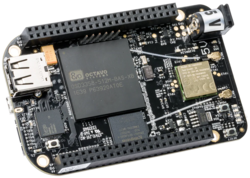
\includegraphics[width=5cm]{../slides/beagleboneblack-board/beagleboneblack_sd.png}
  \end{center}
}

\defboard
{beagleplay}
{BeaglePlay}
{
  {\bf BeaglePlay} board
  \begin{itemize}
    \item Texas Instruments AM625x (4xARM Cortex-A53 CPU)
    \item SoC with 3D acceleration, integrated MCU and many other peripherals.
    \item 2 GB of RAM
    \item 16 GB of on-board eMMC storage
    \item USB host and USB device, microSD, HDMI
    \item 2.4 and 5 GHz WiFi, Bluetooth and also Ethernet
    \item 1 MicroBus Header (SPI, I2C, UART, ...), OLDI and CSI connector.
  \vspace{-0.7cm}
  \end{itemize}
}
{BeaglePlay}
{
  Carte {\bf BeaglePlay}
  \begin{itemize}
    \item SoC Texas Instruments AM625x (CPU 4xARM Cortex-A53)
    \item SoC avec accélération 3D, MCU intégré et de nombreux autres périphériques.
    \item 2 GB de RAM
    \item 16 Go de stockage eMMC
    \item USB hôte et device, microSD, HDMI
    \item WiFi 2.4 and 5 GHz, Bluetooth et aussi Ethernet
    \item 1 Header MicroBus (SPI, I2C, UART, ...), connecteurs OLDI et CSI.
  \vspace{-0.7cm}
  \end{itemize}
}
{
  \begin{center}
    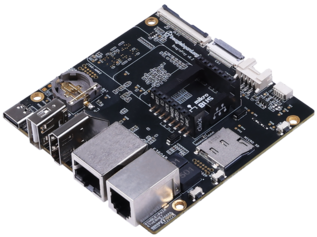
\includegraphics[width=5cm]{../slides/beagleplay-board/beagleplay_sd.png}
  \end{center}
}

\defboard
{espressobin}
{Hardware platform for practical labs}
{
  {\bf Globalscale EspressoBin} board
  \begin{itemize}
  \item Dual Cortex A53 Marvell Armada 3720 SoC
  \item Onboard switch with 2x 1Gbps interfaces
  \item Extra 1Gbps interface
  \item 1GB RAM
  \item 1x SATA interface
  \item 1x USB 3.0 interface
  \end{itemize}
}
{Plateforme matérielle pour les travaux pratiques}
{
  Carte {\bf Globalscale EspressoBin}
  \begin{itemize}
  \item SoC Marvell Armada 3720 SoC (CPU 2xARM Cortex A53)
  \item Switch Ethernet avec 2 interfaces Gigabit
  \item Interface Gigabit Ethernet additionnelle
  \item 1GB de RAM
  \item 1x interface SATA
  \item 1x interface USB 3.0
  \end{itemize}
}
{
  \begin{center}
    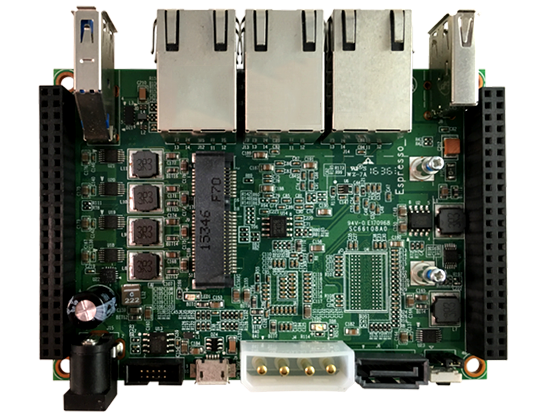
\includegraphics[width=5cm]{../slides/espressobin/espressobin.png}
  \end{center}
}


\def \training{audio}

% Title
\ifthenelse{\equal{\agendalanguage}{french}}{
  \def \trainingtitle{Formation Comprendre la stack audio sous Linux embarqué}
}{
  \def \trainingtitle{Audio with embedded Linux training}
}

% Duration
\ifthenelse{\equal{\trainingtype}{online}}{
  \def \trainingduration{4}
}{
  \def \trainingduration{2}
}

% Training objectives
\ifthenelse{\equal{\agendalanguage}{french}}{
  \def \traininggoals{
    \begin{itemize}
    \item Être capable de comprendre les bases de la théorie audio:
      analogique vs. numérique, échantillonage, formats audio,
      composants matériels audio
    \item Être capable de comprendre l'architecture de ASoC, le
      sous-système du noyau Linux pour les périphériques audio des
      systèmes embarqués, le rôle des différents drivers et la
      représentation Device Tree correspondante
    \item Être capable d'écrire un Device Tree décrivant la topologie
      des composants matériels audio dans un système Linux embarqué
    \item Être capable d'utiliser des possibilités de routage audio
      avancées, la gestion de l'énergie audio et des composants audio
      complexes tels que les périphériques auxilliaires et les
      amplificateurs
    \item Être capable de configurer les composants ALSA en espace
      utilisateur et les widgets ALSA
    \item Être capable de mettre en oeuvre les différentes APIs en
      espace utilisateur pour la lecture et l'enregistrement audio,
      ainsi que le serveur audio PipeWire et le framework multimedia
      GStreamer
    \end{itemize}
  }
}{
  \def \traininggoals{
    \begin{itemize}
    \item Be able to understand the basics of audio theory: analog
      vs. digital, sampling theory, audio formats and audio hardware
    \item Be able to understand the architecture of ASoC, the Linux
      kernel subsystem for audio devices used in embedded systems, the
      role of the different drivers and the Device Tree representation
    \item Be able to write a Device Tree describing the topology of
      audio hardware on an embedded Linux system
    \item Be able to use complex audio routing capabilities, audio power
      management capabilities, and complex audio components such as
      auxiliary devices or amplifiers
    \item Be able to configure the ALSA user-space components and
      ALSA audio widgets
    \item Be able to use the available user-space APIs for playing and
    capturing audio, as well as the PipeWire audio server and the
    GStreamer multimedia pipeline library
  \end{itemize}
}
}

% Training prerequisites
\def \trainingprerequisites{
  \begin{itemize}
    \prerequisitecommandline
    \prerequisiteembeddedlinux
    \prerequisiteenglish
  \end{itemize}
}

% Training audience
\ifthenelse{\equal{\agendalanguage}{french}}{
  \def \trainingaudience{
    Ingénieurs qui ont besoin d'une compréhension en détail des
    concepts audio, des composants matériels utilisés pour l'audio
    dans les systèmes embarqués et du fonctionnement de la stack audio
    sous Linux.
  }
}{
  \def \trainingaudience{
    Engineers who need a detailed level of understanding of audio
    concepts, audio hardware components used in typical embedded
    systems and how the audio stack works in Linux.
  }
}

% Required equipment on-site
\ifthenelse{\equal{\trainingtype}{onsite}}{
  \ifthenelse{\equal{\agendalanguage}{french}}{
    \def \requiredequipment {
      {\bf Pour les sessions en présentiel dans les locaux de nos clients,
        notre client doit fournir}:
      \begin{itemize}
      \item Projecteur vidéo
      \item Un grand moniteur
      \item Un tableau pour écrire
      \end{itemize}
    }
  }{
    \def \requiredequipment {
      {\bf For on-site sessions at our customer location, the customer must provide}:
      \begin{itemize}
      \item Video projector
      \item Large monitor
      \item Drawing board
      \end{itemize}
    }
  }
}{}

% No labs in audio course
\def \haslabs{false}

% Time ratio
\def \onsitelecturetimeratio{75}
\def \onsitedemotimeratio{25}

% Agenda items

\defagendaitem
{representation}
{lecture}
{Digital Audio Representation}
{
  \begin{itemize}
  \item What is sound?
  \item Sampling theory
  \item Sample size, sample rate
  \item Audio formats: I2S, LJ, RJ, DSPA, DSPB
  \item AC97
  \item IEC 61937 (S/PDIF and HDMI)
  \item PDM
  \end{itemize}
  \vspace{0.5em}
  {\em Introducing the basic notions used for representing audio waveforms.}
}
{Représentation audio numérique}
{
  \begin{itemize}
  \item Qu'est-ce que le son?
  \item Théorie de l'échantillonage
  \item Taille des échantillons, fréquence d'échantillonage
  \item Formats audio : I2S, LJ, RJ, DSPA, DSPB
  \item AC97
  \item IEC 61937 (S/PDIF and HDMI)
  \item PDM
  \end{itemize}
  \vspace{0.5em}
  {\em Introduction des notions de base utilisées pour représenter des ondes audio.}
}
\defagendaitem
{hardware}
{lecture}
{Hardware}
{
  \begin{itemize}
  \item Signals
  \item CPU Digital Audio Interfaces
  \item CODEC Digital Audio Interfaces
  \item Amplifiers
  \item Clocks and clock providers
  \end{itemize}
  \vspace{0.5em}
  {\em Presenting the hardware involved in the audio playback or capture.}
}
{Matériel}
{
  \begin{itemize}
  \item Signaux
  \item Interfaces audio numériques sur les System-on-chip
  \item Interfaces audio numériques sur les codecs audio
  \item Amplificateurs
  \item Horloges et fournisseurs d'horloges
  \end{itemize}
  \vspace{0.5em}
  {\em Présentation du matériel impliqué dans la lecture ou l'enregistrement audio.}
}
\defagendaitem
{asoc}
{lecture}
{Linux kernel ASoC subsystem}
{
  \begin{itemize}
  \item ASoC: the ALSA System-on-Chip subsystem in the Linux kernel
  \item Describing audio cards with Device Tree: {\em
      audio-graph-card}, {\em simple-audio-card}
  \item Linux kernel drivers for audio cards
  \item Linux kernel drivers for audio codecs
  \item Controls
  \item Linux kernel drivers for CPU audio interfaces
  \end{itemize}
  \vspace{0.5em}
  {\em Introducing the Linux kernel subsystem for audio on embedded systems.}
}
{Le sous-système ASoC du noyau Linux}
{
  \begin{itemize}
  \item ASoC : le sous-système ALSA pour les System-on-chip dans le noyau Linux
  \item Description des cartes audio dans le Device Tree : {\em
      audio-graph-card}, {\em simple-audio-card}
  \item Drivers dans le noyau Linux pour les cartes audio
  \item Drivers dans le noyau Linux pour les codecs audio
  \item Controles audio dans le kernel
  \item Drivers dans le noyau Linux pour les interfaces audio des
    System-on-chip
  \end{itemize}
  \vspace{0.5em}
  {\em Introduction au sous-système du noyau Linux pour la gestion audio dans les systèmes embarqués.}
}
\defagendaitem
{kernelhelpers}
{lecture}
{Linux kernel helpers}
{
  \begin{itemize}
  \item {\em regmap}, {\em regcache}
  \item DMA handling
  \end{itemize}
  \vspace{0.5em}
  {\em Presenting the common helper APIs.}
}
{Mécanismes supplémentaires du noyau Linux relatifs à l'audio}
{
  \begin{itemize}
  \item {\em regmap}, {\em regcache}
  \item Support DMA
  \end{itemize}
  \vspace{0.5em}
  {\em Présentation des mécanismes du noyau Linux couramment utilisés en lien avec le support audio.}
}
\defagendaitem
{audiocomponents}
{lecture}
{More audio components}
{
  \begin{itemize}
  \item Auxiliary devices, amplifiers, muxing
  \item Jack detection
  \item Asynchronous Sample Rate Converter
  \end{itemize}
  \vspace{0.5em}
  {\em Presenting more components of the sound cards.}
}
{Autres composants audio}
{
  \begin{itemize}
  \item Périphériques auxilliaires, amplificateurs, muxing
  \item Detection Jack
  \item Convertisseur de fréquence d'échantillonage asynchrone
  \end{itemize}
  \vspace{0.5em}
  {\em Présentation de composants supplémentaires utilisés pour certaines cartes audio.}
}
\defagendaitem
{routing}
{lecture}
{Routing}
{
  \begin{itemize}
  \item Routing audio
  \item DAPM: Dynamic Audio Power Management
  \end{itemize}
  \vspace{0.5em}
  {\em Presenting the audio routes and power management.}
}
{Routage}
{
  \begin{itemize}
  \item Routage de flux audio
  \item DAPM : {\em Dynamic Audio Power Management}
  \end{itemize}
  \vspace{0.5em}
  {\em Présentation du routage audio et de la gestion d'énergie pour l'audio.}
}
\defagendaitem
{userspacehardwareconfiguration}
{lecture}
{Userspace, hardware configuration}
{
  \begin{itemize}
  \item ALSA plugins
  \item \code{asound.conf}
  \item Sound card configuration
  \end{itemize}
  \vspace{0.5em}
  {\em Configuring the userspace audio paths and effects.}
}
{Espace utilisateur et configuation matérielle}
{
  \begin{itemize}
  \item Plug-ins ALSA
  \item \code{asound.conf}
  \item Configuration de cartes son en espace utilisateur
  \end{itemize}
  \vspace{0.5em}
  {\em Configuration des chemins et effets audio depuis l'espace utilisateur.}
}
\defagendaitem
{userspacehardwareconfiguration}
{lab}
{Card configuration examples}
{
  \begin{itemize}
  \item Reordering channels
  \item Splitting channels
  \item Resampling
  \item Mixing
  \item LADSPA
  \end{itemize}
  \vspace{0.5em}
  {\em Exercising the ALSA plugins.}
}
{Exemples de configuration de cartes audio}
{
  \begin{itemize}
  \item Changement d'ordre des canaux audio
  \item Séparation de canaux audio
  \item Ré-échantillonage
  \item Mixing
  \item LADSPA
  \end{itemize}
  \vspace{0.5em}
  {\em Mise en oeuvre des plug-ins ALSA}
}
\defagendaitem
{userspacecontrolconfiguration}
{lecture}
{Userspace, controls configuration}
{
  \begin{itemize}
  \item {\em amixer}
  \item {\em alsamixer}
  \item Userspace API
  \item Saving state: {\em alsactl}, \code{asound.state}
  \end{itemize}
  \vspace{0.5em}
  {\em Configuring the userspace audio paths and effects.}
}
{Espace utilisateur et configuration des contrôles audio}
{
  \begin{itemize}
  \item {\em amixer}
  \item {\em alsamixer}
  \item API en espace utilisateur
  \item Sauvegarde de l'état des contrôles : {\em alsactl}, \code{asound.state}
  \end{itemize}
  \vspace{0.5em}
  {\em Configuration des chemins et effets audio depuis l'espace utilisateur.}
}
\defagendaitem
{userspacecontrolconfiguration}
{lab}
{Configuring controls}
{
  \begin{itemize}
  \item {\em alsamixer} demonstration
  \item \code{asound.state} examples
  \item Custom application
  \end{itemize}
  \vspace{0.5em}
  {\em Configuring the sound card controls.}
}
{Configuration des contrôles}
{
  \begin{itemize}
  \item TPnstration de {\em alsamixer}
  \item Exemples de fichiers \code{asound.state}
  \item Application custom
  \end{itemize}
  \vspace{0.5em}
  {\em Configuration des contrôles de cartes audio.}
}
\defagendaitem
{userspaceplayaudio}
{lecture}
{Userspace, playing and capturing audio}
{
  \begin{itemize}
  \item Userspace ALSA API
  \end{itemize}
  \vspace{0.5em}
  {\em Playing and capturing audio samples.}
}
{Espace utilisateur : lecture et enregistrement audio}
{
  \begin{itemize}
  \item API de ALSA en espace utilisateur
  \end{itemize}
  \vspace{0.5em}
  {\em Lecture et enregistrement de samples audio}
}
\defagendaitem
{troubleshooting}
{lecture}
{Troubleshooting}
{
  \begin{itemize}
  \item Debugging
  \item {\em vizdapm}
  \end{itemize}
  \vspace{0.5em}
  {\em Presenting how to debug common issues.}
}
{Résolution de problèmes}
{
  \begin{itemize}
  \item Résolution de problèmes courants
  \item {\em vizdapm}
  \end{itemize}
  \vspace{0.5em}
  {\em Présentation de la résolution de problèmes courants.}
}
\defagendaitem
{debugging}
{lab}
{Debugging}
{
  \begin{itemize}
  \item Examples of common issues and their resolutions
  \end{itemize}
}
{Résolution de problèmes}
{
  \begin{itemize}
  \item Exemples de problèmes courants et leur résolution.
  \end{itemize}
}
\defagendaitem
{pipewire}
{lecture}
{Pipewire}
{
  \begin{itemize}
  \item Pipewire introduction
  \item Pipewire configuration
  \item Pipewire tools (pwdump, pw-cli, ...)
  \item Pipewire session and policy management
  \item Pipewire modules and filtering
  \item {\em WirePlumber}
  \end{itemize}
  \vspace{0.5em}
  {\em Using Pipewire as the sound server.}
}
{Pipewire}
{
  \begin{itemize}
  \item Introduction à Pipewire
  \item Configuration de Pipewire
  \item Outils autour de Pipewire (pwdump, pw-cli, ...)
  \item Gestion de session et de {\em policy} avec Pipewire
  \item Modules de Pipewire et filtrage
  \item {\em WirePlumber}
  \end{itemize}
  \vspace{0.5em}
  {\em Utiliser Pipewire comme serveur audio.}
}
\defagendaitem
{pipewire}
{lab}
{Pipewire}
{
  \begin{itemize}
  \item Running pipewire on the target
  \item Inspecting the configuration and setting properties
  \item Dynamic routing and patchbay
  \item Using modules and Filter-Chain
  \end{itemize}
  \vspace{0.5em}
  {\em Running Pipewire and exercising advanced configuration.}
}
{Pipewire}
{
  \begin{itemize}
  \item Lancer pipewire sur une cible embarquée
  \item Inspecter la configuration et les propriétés
  \item Routage dynamique et {\em patchbay}
  \item Utilisation des modules et de {\em Filter-Chain}
  \end{itemize}
  \vspace{0.5em}
  {\em Utiliser Pipewire et des configurations avancées.}
}
\defagendaitem
{gstreamer}
{lecture}
{The GStreamer multimedia framework}
{
  \begin{itemize}
  \item {\em GStreamer}
  \item GStreamer pipelines
  \item GStreamer plugins
  \end{itemize}
  \vspace{0.5em}
  {\em Using Gstreamer for audio capture and playback.}
}
{Le framework multimedia GStreamer}
{
  \begin{itemize}
  \item {\em GStreamer}
  \item Pipelines GStreamer
  \item Plugins GStreamer
  \end{itemize}
  \vspace{0.5em}
  {\em Utiliser GStreamer pour la lecture et l'enregistrement audio.}
}
\defagendaitem
{gstreamer}
{lab}
{GStreamer}
{
  \begin{itemize}
  \item Running gstreamer on the target
  \item Creating multiple pipelines
  \end{itemize}
  \vspace{0.5em}
  {\em Running Gstreamer using different audio pipelines.}
}
{GStreamer}
{
  \begin{itemize}
  \item Lancer gstreamer sur une cible embarquée
  \item Créer différents pipelines
  \end{itemize}
  \vspace{0.5em}
  {\em Exécuter Gstreamer et utiliser différents pipelines audio.}
}

\def \onlineagenda {
  \showonlineagendaday{1}
  \showagendaitem{representation}{lecture}
  \showagendaitem{hardware}{lecture}
  \showagendaitem{asoc}{lecture}
  \showonlineagendaday{2}
  \showagendaitem{kernelhelpers}{lecture}
  \showagendaitem{audiocomponents}{lecture}
  \showagendaitem{routing}{lecture}
  \showonlineagendaday{3}
  \showagendaitem{userspacehardwareconfiguration}{lecture}
  \showagendaitem{userspacehardwareconfiguration}{lab}
  \showagendaitem{userspacecontrolconfiguration}{lecture}
  \showagendaitem{userspacecontrolconfiguration}{lab}
  \showagendaitem{userspaceplayaudio}{lecture}
  \showonlineagendaday{4}
  \showagendaitem{troubleshooting}{lecture}
  \showagendaitem{debugging}{lab}
  \showagendaitem{pipewire}{lecture}
  \showagendaitem{pipewire}{lab}
  \showagendaitem{gstreamer}{lecture}
  \showagendaitem{gstreamer}{lab}
}

\def \onsiteagenda {
  \showonlineagendaday{1}
  \showagendaitem{representation}{lecture}
  \showagendaitem{hardware}{lecture}
  \showagendaitem{asoc}{lecture}
  \showonlineagendaday{2}
  \showagendaitem{kernelhelpers}{lecture}
  \showagendaitem{audiocomponents}{lecture}
  \showagendaitem{routing}{lecture}
  \showonlineagendaday{3}
  \showagendaitem{userspacehardwareconfiguration}{lecture}
  \showagendaitem{userspacehardwareconfiguration}{lab}
  \showagendaitem{userspacecontrolconfiguration}{lecture}
  \showagendaitem{userspacecontrolconfiguration}{lab}
  \showagendaitem{userspaceplayaudio}{lecture}
  \showonlineagendaday{4}
  \showagendaitem{troubleshooting}{lecture}
  \showagendaitem{debugging}{lab}
  \showagendaitem{pipewire}{lecture}
  \showagendaitem{pipewire}{lab}
  \showagendaitem{gstreamer}{lecture}
  \showagendaitem{gstreamer}{lab}
}

